\section{Kiến trúc BERT}
Kiến trúc của BERT -- Bidirectional Encoder Representations from Transformers -- là một minh chứng điển hình cho sự kết hợp hài hòa giữa chiều sâu hình thức toán học và trực giác ngôn ngữ học. Là một mô hình \textbf{encoder-only} được phát triển trên nền tảng của Transformer, BERT được thiết kế để hấp thụ ngữ nghĩa không tuyến tính của ngôn ngữ tự nhiên bằng cách cho phép các biểu diễn ngữ cảnh hóa toàn diện theo cả hai chiều: từ trái sang phải và từ phải sang trái. Chính đặc tính này -- \textbf{bidirectionality} -- đã mở ra một kỷ nguyên mới trong xử lý ngôn ngữ, vượt khỏi giới hạn của các mô hình ngôn ngữ truyền thống vốn mang tính đơn phương.

BERT gồm nhiều tầng encoder được sắp xếp tuần tự, trong đó mỗi tầng là một sự hòa phối của hai thành phần cơ bản: \textbf{multi-head self-attention} và \textbf{feed-forward neural network (FFN)}. Bên trong mỗi tầng attention, thông tin từ mỗi token không chỉ được truyền qua một luồng đơn, mà được phân phối qua nhiều ``đầu'' (head) chú ý song song, mỗi head học cách tập trung vào một khía cạnh khác nhau của ngữ cảnh -- có thể là cú pháp, đồng tham chiếu, hoặc các mối liên hệ ngữ nghĩa trừu tượng hơn. Cơ chế attention này bắt đầu bằng việc tạo ba vector con từ mỗi token: \textbf{Query (Q)}, \textbf{Key (K)} và \textbf{Value (V)}, thông qua các biến đổi tuyến tính. Điểm nổi bật nằm ở phép nhân vô hướng giữa Q và K, được chuẩn hóa theo căn bậc hai của kích thước chiều không gian \(d_k\), sau đó đi qua hàm softmax để tạo ra một phân phối chú ý có tổng bằng 1. Kết quả cuối cùng là tổ hợp có trọng số của các vector V, tạo thành sự phản hồi ngữ nghĩa từ toàn bộ chuỗi đầu vào cho mỗi token riêng lẻ.

\begin{equation}
    Attention(Q, K, V) = softmax\left(\frac{QK^{T}}{\sqrt{d_{k}}}\right) \cdot V
\end{equation}

Sau đó, các output của các head attention được liên kết lại (concatenated) và đưa qua một tầng biến đổi tuyến tính cuối cùng để tạo ra biểu diễn tổng hợp. Mỗi tầng attention đều được bao bọc bởi một \textbf{residual connection} và \textbf{layer normalization}, nhằm ổn định gradient và thúc đẩy quá trình học. Phía sau attention là một mạng FFN với hai lớp tuyến tính, trong đó lớp ẩn thường có kích thước lớn gấp bốn lần kích thước ẩn của mô hình -- ví dụ, từ 768 đến 3072 trong BERT base -- và sử dụng hàm kích hoạt phi tuyến như ReLU để tăng cường khả năng biểu diễn phi tuyến.

Ngoài ra, đầu vào của BERT là tổng của ba loại embedding: \textbf{token embedding} từ từ điển WordPiece (\~30.000 mục từ), \textbf{segment embedding} để phân biệt giữa các câu trong tác vụ NSP (Next Sentence Prediction), và \textbf{position embedding} để giữ thông tin về vị trí tương đối của token trong chuỗi. Tổng thể này tạo nên một biểu diễn đầu vào dày đặc, giàu ngữ cảnh và đầy đủ cấu trúc.

Khác với transformer nguyên bản, BERT loại bỏ cơ chế attention che mặt (masked attention) ở phần decoder, thay vào đó cho phép attention mở rộng toàn phần trong encoder, từ đó học các biểu diễn ngữ nghĩa dựa trên toàn bộ chuỗi đầu vào. Đây là điểm then chốt tạo nên sức mạnh đặc biệt của BERT trong các tác vụ như truy xuất thông tin, phân loại văn bản và trả lời câu hỏi, khi mà ngữ nghĩa của một từ chỉ thực sự hiện hình trong mối tương quan với những từ vây quanh nó -- trước và sau.

\begin{figure}[H]
    \caption{Minh họa kiến trúc BERT}
    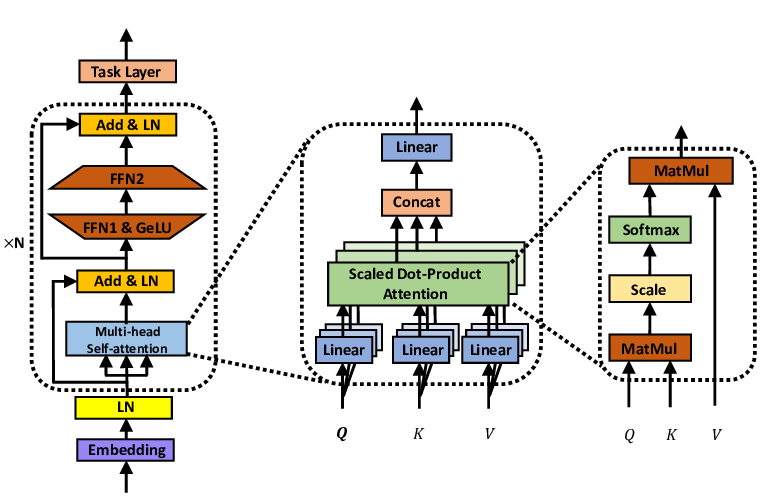
\includegraphics[width=\linewidth]{assets/bert.png}
\end{figure}

Như một bản giao hưởng cấu trúc giữa hình học và ngôn ngữ học, kiến trúc của BERT không chỉ đơn thuần là một mạng học sâu, mà là một không gian ngữ nghĩa nơi mỗi token được tái định nghĩa theo cách nhìn toàn cục. Với khả năng học từ văn bản thô thông qua cơ chế attention đa chiều, BERT đã đặt nền móng cho hàng loạt ứng dụng downstream, khẳng định mình như một trong những trụ cột vững chắc của thời đại học biểu diễn trong xử lý ngôn ngữ tự nhiên.
